% Author: Izaak Neutelings (February 2020)
\documentclass[border=10pt,tikz]{standalone}
\usepackage{physics}
\usepackage{xcolor}
\usetikzlibrary{decorations.markings}
\tikzset{>=latex} % for LaTeX arrow head

\colorlet{Ecol}{orange!90!black}
\colorlet{Bcol}{violet!90}
\colorlet{Icol}{blue!70!black}
\colorlet{gausscol}{green!40!black}
\colorlet{gausscol2}{green!45!blue}
\tikzstyle{current}=[->,Icol,thick]
\colorlet{pluscol}{red!60!black}
\colorlet{minuscol}{blue!60!black}
\tikzstyle{anode}=[top color=red!20,bottom color=red!50,shading angle=20]
\tikzstyle{cathode}=[top color=blue!20,bottom color=blue!40,shading angle=20]
\tikzstyle{gauss surf}=[gausscol,top color=green!2,bottom color=green!80!black!70,shading angle=5,fill opacity=0.4]
\tikzstyle{metal}=[top color=black!15,bottom color=black!25,middle color=black!20,shading angle=10]
\tikzstyle{mydashes}=[dash pattern=on 1 off 1]
\tikzset{
  EFieldLine/.style={thick,Ecol,line cap=round,decoration={markings,
                     mark=at position #1 with {\arrow{latex}}},
                     postaction={decorate}},
  BFieldLine/.style={thick,Bcol,postaction={decorate},decoration={markings,
                     mark=at position #1 with {\arrow{latex}},
                     mark=at position #1+0.5 with {\arrow{latex}}}},
  EFieldLine/.default=0.5,
  BFieldLine/.default=0.4}
\usetikzlibrary{3d}

\begin{document}


% CAPACITOR 3D - displacement current derivation
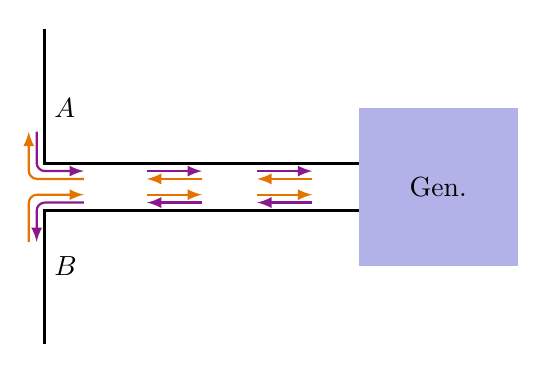
\begin{tikzpicture}[]
    \def\RC{1.2}     % radius capacitor
    \def\RW{0.1*\RC} % radius wire
    \def\RA{1.6}     % radius ampere loop
    \def\D{2.6*\RA}  % distance between plates
    \def\T{0.4}      % plate thickness
    \def\L{2*\RA}    % wire length
    \def\NE{5}       % number of electric field lines
    \def\NB{2}       % number of magnetic field lines
    
    \draw [very thick](0, 2) -- (0, 0.3) -- (4, 0.3);
    \draw [very thick](0, -2) -- (0, -0.3) -- (4, -0.3);
    \filldraw [color = Icol!30] (4, -1) rectangle ++ (2, 2);
    \draw[rounded corners=3pt, Bcol, thick, -latex] (-0.1, 0.7) -- (-0.1,0.2) -- (0.5,0.2);
    \draw[rounded corners=3pt, Bcol, thick, -latex] (1.3, 0.2) -- (2.0,0.2) ;
    \draw[rounded corners=3pt, Bcol, thick, -latex] (2.7, 0.2) -- (3.4,0.2) ;
    \draw[rounded corners=3pt, Bcol, thick, latex-] (2.7, -0.2) -- (3.4,-0.2) ;
    \draw[rounded corners=3pt, Bcol, thick, -latex] (2.0, -0.2) -- (1.3,-0.2) ;
    \draw[rounded corners=3pt, Bcol, thick, latex-] (-0.1, -0.7) -- (-0.1,-0.2) -- (0.5,-0.2);

    \draw[rounded corners=3pt, Ecol, thick, latex-] (-0.2, 0.7) -- (-0.2,0.1) -- (0.5,0.1);
    \draw[rounded corners=3pt, Ecol, thick, latex-] (1.3, 0.1) -- (2.0,0.1) ;
    \draw[rounded corners=3pt, Ecol, thick, latex-] (2.7, 0.1) -- (3.4,0.1) ;
    \draw[rounded corners=3pt, Ecol, thick, -latex] (2.7, -0.1) -- (3.4,-0.1) ;
    \draw[rounded corners=3pt, Ecol, thick, latex-] (2.0, -0.1) -- (1.3,-0.1) ;
    \draw[rounded corners=3pt, Ecol, thick, -latex] (-0.2, -0.7) -- (-0.2,-0.1) -- (0.5,-0.1);
    \node [right] at (0, 1) {$A$};
    \node [right] at (0, -1) {$B$};
    \node [align=center] at (5, 0) {Gen.};
\end{tikzpicture}
  
\end{document}